\section{Grundlagen}\label{sec:Grundlagen}
\subsection{Signalvorverarbeitung}
Um ein gegebenes Audiosignal einheitlich verarbeiten zu können, muss dieses zunächst mittels verschiedener Verfahren vorbereitet werden.
Ziel dieser Vorverarbeitung ist es, die Effizienz und Effektivität des anschließenden Verarbeitungsprozess zu erhöhen und somit ein verbessertes Ergebnis zu erzielen \autocite[vgl.][S. 11672]{lokesh_speech_2019}.
Die Vorverarbeitung im Rahmen dieser Arbeit beschränkt sich auf die beiden Schritte Framing und Windowing, welche in den folgenden Unterkapiteln genauer erläutert werden.

\subsubsection{Framing}
Das Unterteilen von Audiosignalen in kleinere Blöcke (Frames) wird als Framing bezeichnet.
Dabei muss zunächst eine einheitliche Blockgröße festgelegt werden.
Außerdem wird eine Überlagerungszeit definiert, welche eine Überlappung der einzelnen Blöcke verursacht.
% TODO: Quelle hinzufügen
% TODO: Warum wird überlagert -> Quelle

\subsubsection{Windowing (Zeitfenster)}
\begin{figure}
  \centering
  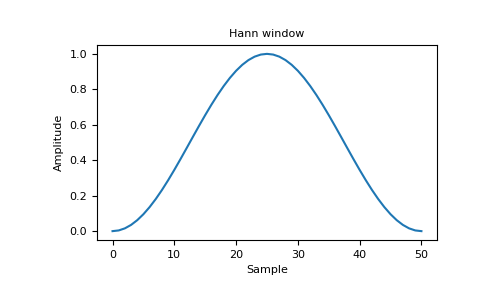
\includegraphics[width=0.8\textwidth, keepaspectratio]{images/hann_window.png}
  \caption{Von Hann Fensterfunktion \autocite{noauthor_numpyhanning_nodate}}
  \label{fig:vonHannFenster}
\end{figure}
Um die bei der Unterteilung des Audiosignals entstandenen Diskontinuitäten aufzulösen, wird eine Fensterfunktion auf die einzelnen Blöcke angewendet.
Abbildung~\ref{fig:vonHannFenster} zeigt die von Hann Fensterfunktion, welche neben dem Hamming Fenster zu den typischen Fensterfunktionen in der Audiosignalverarbeitung zählt.
Durch den Nulldurchgang am Anfang und Ende der Fensterfunktion werden die Amplituden des Blocksignals nach Anwenden der Funktion an den Grenzen auf Null gezogen, wodurch sich ein kontinuierlicher, periodischer Signalverlauf ergibt.
Dieser wird von den in dieser Arbeit verwendeten Funktionen wie etwa der \ac{FFT} vorausgesetzt.

Wird der Schritt des Windowing nicht durchgeführt, führt dies zu einem Phänomen namens Spectral leakage.
Der Amplitudensprung an den Blockenden resultiert in der Registrierung einer vielzahl von Frequenzen, welches die korrekte Ermittlung der sich im Signal befindenden Frequenzen erschwert.
Wie der Name bereits beschreibt, wird aus einer eindeutigen Frequenz, ein Spektrum aus Frequenzen.
% TODO: Wird Windowing in diesem Anwendungsfall überhaupt benötigt?

\begin{itemize}
  \item Spektral leakage
  \item Hamming und Han Fenster
  \item Unterschied zu Framing
\end{itemize}
\subsection{Auto regressive moving average filter}
% TODO: Was ist es + was hat es mit LPC zu tun

\subsection{Cepstral vectors/coefficients}
% TODO: Was sind Cepstral coefficients
% TODO: Warum werden sie verwendet, was ist der Vorteil?
